\documentclass[12pt, twoside, letterpaper]{report}
\usepackage[top=2cm,bottom=4cm,left=3cm,right=3cm,asymmetric]{geometry}

\usepackage{fancyhdr}
\pagestyle{fancy}
\fancyfoot[C]{}    
\fancyfoot[LE,RO]{\thepage}        
\fancyhead[RO]{\slshape \rightmark}        
\fancyhead[LE]{\slshape\leftmark}      
\fancyhead[RE,LO]{}  

\usepackage{color}   
\usepackage{hyperref}
\usepackage[utf8x]{inputenc}
\usepackage[english]{babel}
\usepackage{amsmath, amsthm, amssymb, amsfonts}
\usepackage[breakable]{tcolorbox}
\usepackage{pdfpages}
\usepackage{graphicx}
\graphicspath{ {./img/} }

\title{Uso di reti neurali per la classificazione di dati in problemi di medicina legale}
\author{Mario Petruccelli \cr Università degli studi di Milano}
\date{A.A. 2019/2020}

\addto\captionsenglish{
	\renewcommand{\contentsname}{Indice}
	\renewcommand{\chaptername}{Capitolo}
}
\addto\captionsenglish{}

\begin{document}

	\begin{titlepage}
		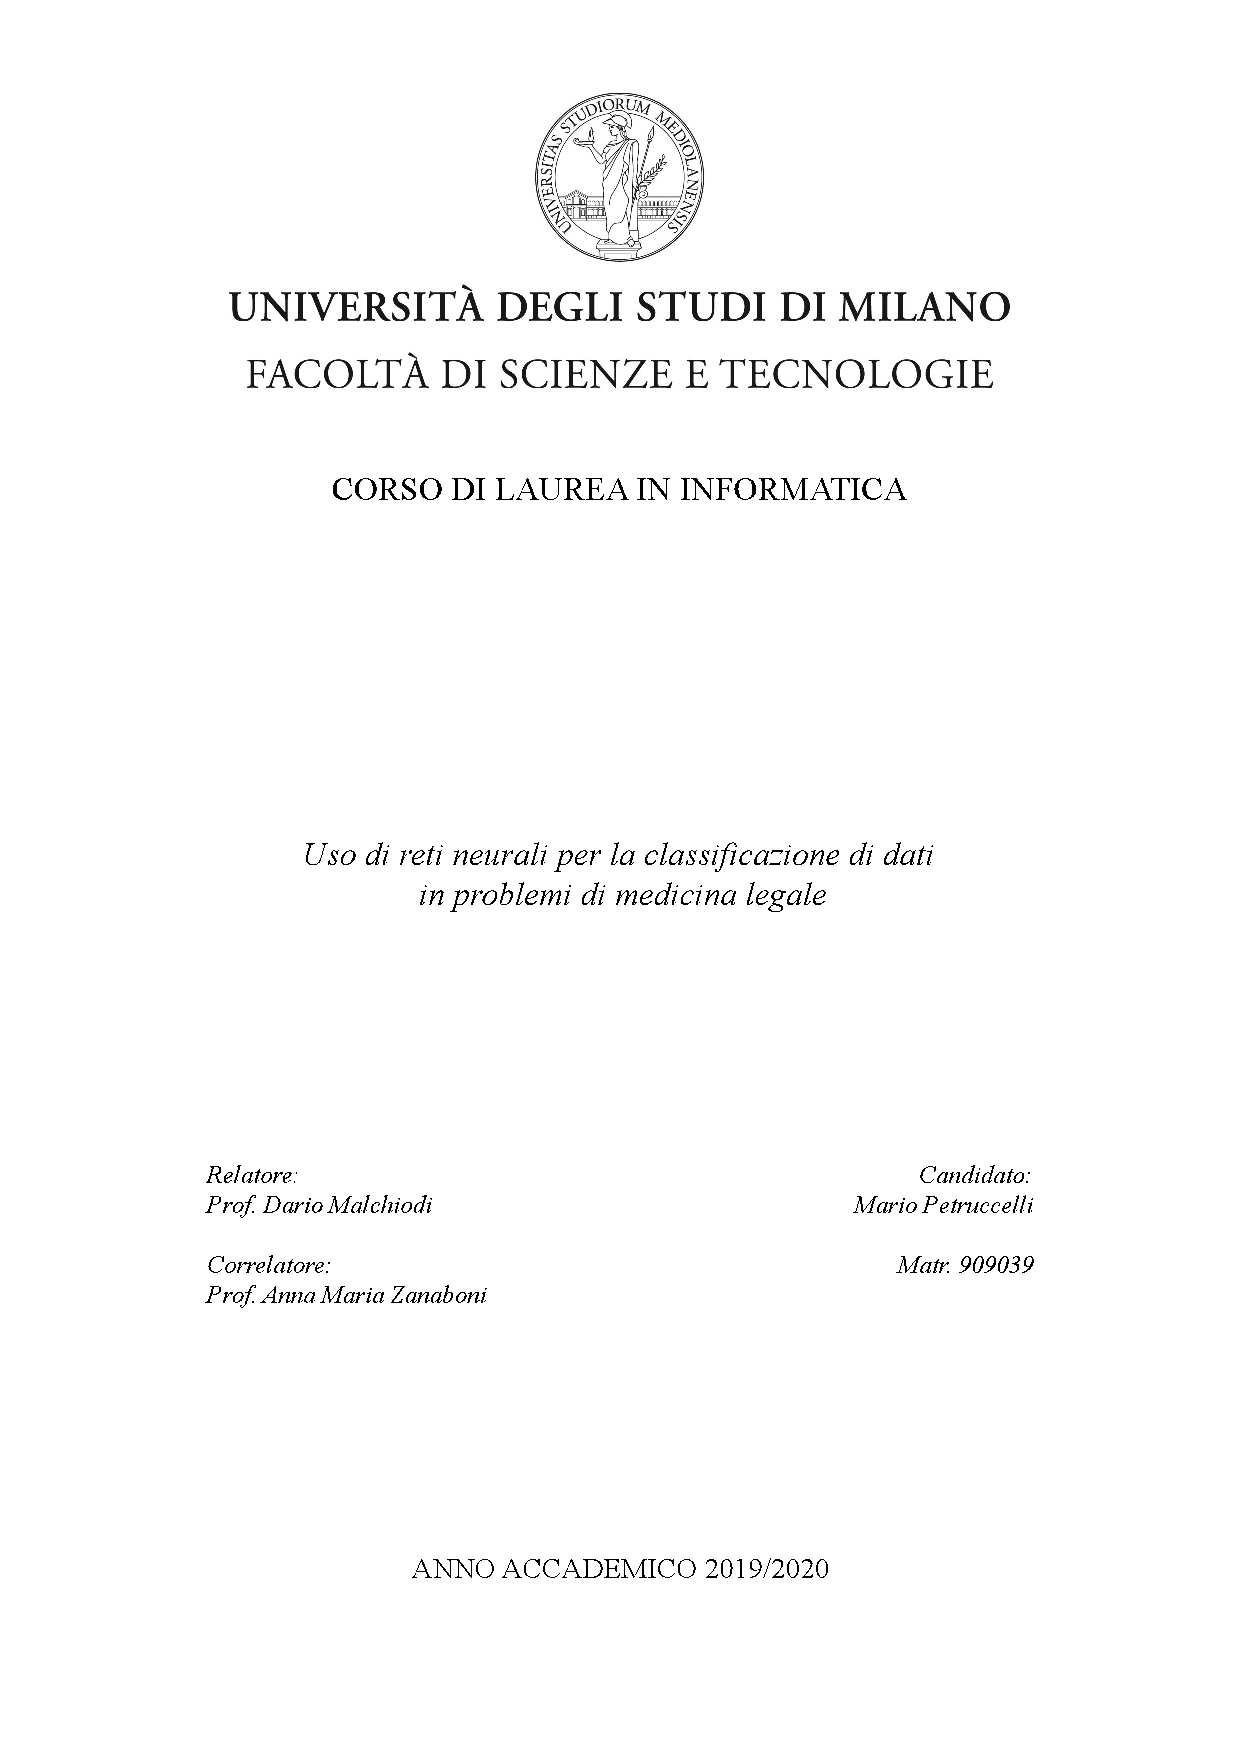
\includepdf{img/FRONTESPIZIO.pdf}
		\newpage
		\tableofcontents
	\end{titlepage}

	\chapter*{Introduzione} \markboth{Introduzione}{}
		Qua ci andrà l'introduzione

		\newpage		
	\chapter{Reti neurali}
		Le \textbf{reti neurali artificiali} sono un campo molto importante del \textit{machine learning}. Consistono in un modello matematico che prende ispirazione dalle reti neurali biologiche, presenti nel cervello animale. In questo capitolo ne vedremo le loro componenti e il loro funzionamento. Ma cos'è il machine learning?

		\section{Paradigma del machine learning}
			Il machine learning è una disciplina scientifica dell'ambito dell'intelligenza artificiale ed è una di quelle in più rapida espansione. Lo scopo di tale disciplina è quello di individuare dei pattern significativi nei dati. Negli ultimi decenni è diventato di uso comune in moltissime applicazioni che richiedono l'estrazione di informazioni da dati su larga scala.
			 
			
		\section{Che cos'è una rete neurale?}
		\section{Componenti principali di una rete neurale}
		\section{Rete neurale feedforward}
		\section{Discesa del gradiente e back propagation}
		
	\chapter{Tecniche utilizzate}
		\section{Preprocessing}
			\subsection{Cross validation}
			\subsection{Grid search CV}
			\subsection{Scalatura dei dati}
		\section{Model Selection}			
			\subsection{Analisi delle componenti principali}
			\subsection{t-distributed Stochastic Neighbor Embedding}
		\section{Over-sampling}
			\subsection{Synthetic Minority Over-sampling Technique}
		
	\chapter{Esperimenti}
		\section{Dataset}
		\section{Esperimenti di classificazione}
		\section{Reingegnerizzazione dei dati}
		\section{Data augmentation}

	\chapter*{Conclusione}	
	
\end{document}



